% cd /disks/PROJECT/Mickael/COMMUNICATION/JTLille2/;
% pdflatex Beamer_JTLille2.tex; bibtex Beamer_JTLille2; pdflatex Beamer_JTLille2.tex; pdflatex Beamer_JTLille2.tex
% evince Beamer_JTLille2.pdf &

\documentclass[10pt, xcolors={RGB}, hyperref={pdfpagelabels=false,
        colorlinks=true,
        pdftex=true,
        bookmarks=true,
        bookmarksopen=true,
        hyperfootnotes=true}]{beamer}
\pdfpageattr{/Group << /S /Transparency /I true /CS /DeviceRGB>>}
\usepackage[T1]{fontenc}
\usepackage[utf8]{inputenc}
\usepackage{graphicx}
\usepackage{tabularx}
\usepackage{multirow}
\usepackage{pifont}
\usepackage{multicol}
\usepackage{setspace}
\renewcommand{\baselinestretch}{1.5}
\usepackage{helvet}
\renewcommand{\familydefault}{\sfdefault}
\usepackage[square, authoryear]{natbib}

\definecolor{dodgerblue}{RGB}{30,144,255}
\definecolor{springgreen3}{RGB}{0,139,69}
\definecolor{springgreen2}{RGB}{0,205,102}
\definecolor{firebrick2}{RGB}{238,44,44}
\definecolor{maroon2}{RGB}{238,48,167}
\definecolor{goldenrod2}{RGB}{238,180,34}
\definecolor{deepskyblue}{RGB}{0,191,255}



\usetheme{CambridgeUS}
\useoutertheme{infolines}
\useinnertheme{rectangles}
\setbeamercolor{frametitle}{fg=white, bg=springgreen3!90!black!60!white}
\setbeamercolor{title}{fg=white, bg=springgreen3!50!white}
\setbeamercolor{palette primary}{fg=springgreen3!40!black, bg=springgreen3!50!white}
\setbeamercolor{palette secondary}{fg=springgreen3!30!black, bg=springgreen3!70!white}
\setbeamercolor{palette tertiary}{fg=springgreen3!20!black, bg=springgreen3!90!white}
\setbeamercolor{structure}{fg=springgreen3!70!white}
\setbeamercolor{background canvas}{bg=white}
\setbeamercolor{normal text}{fg=black}
\setbeamercolor{block title}{bg=dodgerblue, fg=white!75!dodgerblue}
\setbeamercolor{example text}{fg=springgreen3}
\setbeamercolor{block title example}{bg=springgreen3, fg=white!75!springgreen3}
\setbeamercolor{alerted text}{fg=firebrick2}
\setbeamercolor{block title alerted}{bg=firebrick2, fg=white!75!firebrick2}
\setbeamertemplate{navigation symbols}{}
\addtobeamertemplate{headline}{\hypersetup{allcolors=springgreen3!40!black}}{}

\def\cst#1{\def\@cst{#1}}
\defbeamertemplate*{title page}{custom}[1][]{
    \renewcommand{\baselinestretch}{1.25}
    \begin{centering}
        \begin{beamercolorbox}[sep=3pt,center,#1]{institute}
            \usebeamerfont{institute}{\insertinstitute}
        \end{beamercolorbox}
        \vfill
        \begin{beamercolorbox}[sep=8pt, center, colsep=-4bp, rounded=true, shadow=true, #1]{title}
            \usebeamerfont{title}\inserttitle\par%
            \ifx\insertsubtitle\@empty%
            \else%
            \vskip0.25em%
            {\usebeamerfont{subtitle}\usebeamercolor[fg]{subtitle}\insertsubtitle\par}%
            \fi%
        \end{beamercolorbox}%
        \vskip1em\par
        \begin{beamercolorbox}[sep=8pt,center,#1]{author}
            \usebeamerfont{author}\insertauthor
        \end{beamercolorbox}
        \begin{beamercolorbox}[sep=8pt,center,#1]{cst}
            \usebeamerfont{institute}\@cst
        \end{beamercolorbox}
        \begin{beamercolorbox}[sep=8pt,center,#1]{date}
            \usebeamerfont{date}{\small\insertdate}
        \end{beamercolorbox}
        \vfill
        {\usebeamercolor[fg]{titlegraphic}\inserttitlegraphic\par}
    \end{centering}
    \renewcommand{\baselinestretch}{1.5}
}



\hypersetup{%
    linkcolor=dodgerblue,
    urlcolor=firebrick2,
    citecolor=springgreen3,
    filecolor=goldenrod2,
    menucolor=dodgerblue,
    bookmarksopen=true}
\renewcommand{\thefootnote}{\textcolor{maroon2}{\arabic{footnote}}}

\usepackage{textcomp}
\usepackage{listings}
\usepackage{courier}

\newcommand\bref[2]{\hyperref[#1]{#2~\ref*{#1}}}
\newcommand\cmd[1]{\texttt{\color{black}\textbf{#1}}}
\newcommand\cmdb[1]{\texttt{\color{dodgerblue}\textbf{#1}}}
\newcommand\cmdr[1]{\texttt{\color{firebrick2}\textbf{#1}}}
\newcommand\cmdg[1]{\texttt{\color{springgreen3}\textbf{#1}}}
\newcommand\cmdy[1]{\texttt{\color{goldenrod2}\textbf{#1}}}
\newcommand\blue[1]{{\color{dodgerblue}\textbf{#1}}}
\newcommand\red[1]{{\color{firebrick2}\textbf{#1}}}
\newcommand\green[1]{{\color{springgreen3}\textbf{#1}}}
\newcommand\yellow[1]{{\color{goldenrod2}\textbf{#1}}}
\newcommand\pql{{\rmfamily \textbf{\color{goldenrod2}``}}}
\newcommand\pqr{{\rmfamily \textbf{\color{goldenrod2}''}}}
\newcommand\pq[3]{{\rmfamily \textbf{\color{#3}``}}#1{\rmfamily \textbf{\color{#3}''}} - \textcolor{#3}{#2}}
\newenvironment{bquote}[1]
    {\begin{quotation}
    \vspace{10pt}
    \newcommand{\bqauthor}{\normalfont \begin{quote}\begin{flushright}--- #1\end{flushright}\end{quote}}
    \rmfamily \itshape {\huge\textbf{``}}
    }
    {{\huge\textbf{''}}
    \bqauthor
    \end{quotation}
    }

\usepackage[english, francais]{babel}
% \usepackage[english]{babel}
\selectlanguage{francais}

% \AtBeginSection[]
% {
  % \begin{frame}
    % \frametitle{Sommaire}
    % \tableofcontents[sectionstyle=show/hide, subsectionstyle=show/hide/hide]
  % \end{frame}
% }



\usepackage[english, francais]{babel}
\selectlanguage{francais}

\date[\today]{%
    {\color{springgreen3!70!white}\today}
}

\author[Mickaël Canouil]{%
    \texorpdfstring{Mickaël Canouil\\ \vskip -0.25cm
    \href{mailto:mickael.canouil@cnrs.fr}{{\scriptsize mickael.canouil@cnrs.fr}}}{Mickaël Canouil}
}

\institute[CNRS UMR 8199]{%
    {\textcolor{springgreen3!90!white}{\blue{G}énomique \blue{I}ntégrative et \blue{M}odélisation des \blue{M}aladies \blue{M}étaboliques
    \linebreak UMR 8199 (CNRS / Université de Lille 2 / Institut Pasteur de Lille)}}%
}

\titlegraphic{%
    
\includegraphics[height=1cm, keepaspectratio]{../UTILS/Logos/logo_cnrs.pdf}\hspace{1.5cm}
    
\includegraphics[height=1cm, keepaspectratio]{../UTILS/Logos/UL2-WEB-2014.png}\hspace{1.5cm}
    
\includegraphics[height=1cm, keepaspectratio]{../UTILS/Logos/Institut-Pasteur-de-Lille.png}\hspace{1.5cm}
    
\includegraphics[height=1cm, keepaspectratio]{../UTILS/Logos/logo_egid.pdf}%
}
\cst{\textcolor{springgreen3}{Journée Thématique}}

\title[\texorpdfstring{\textcolor{black}{Analyses statistiques et épigénétiques}}{}]{Analyses statistiques et épigénétiques}
\subtitle{%
    % \textit{Sous-titre}
}

\graphicspath{{figures/}}

\usepackage{tikz}
\usebackgroundtemplate{%
    \shorthandoff{;}%
    \tikz\node[opacity=0.20, inner sep=0pt] {
\includegraphics[height=\paperheight, width=\paperwidth]{../UTILS/Background/BG03_Beamer.jpg}};%
}


\begin{document}
\maketitle


\begin{frame}[allowframebreaks]{\blue{\lettrine{I}}ntroduction}
\par{La méthylation de l'ADN joue un rôle important dans la régulation de l'expression des gènes.}
\vspace{1cm}
\par{Une hyper- ou hypo-méthylation importante de l'ADN peut avoir un impact sur l'expression des gènes et être impliqués dans la survenue d'une pathologie et/ou ses complications.}
\framebreak
\par{Afin d'étudier les marques de méthylation, notamment celle des sites CpG, des puces existent et fournissent une mesure quantitative (pourcentage) de la méthylation de ces sites.}
\begin{center}
    \fbox{
\includegraphics[width=7cm]{figures/Capture1.png}}
\end{center}
\vspace{1cm}
\par{Ces puces couvrent 99\% des gènes identifiés et référencés sur RefSeq.}
\framebreak
\par{Les sites CpG sont répartis en différentes régions sur l'ADN: géniques et non géniques.}
\begin{center}
    \fbox{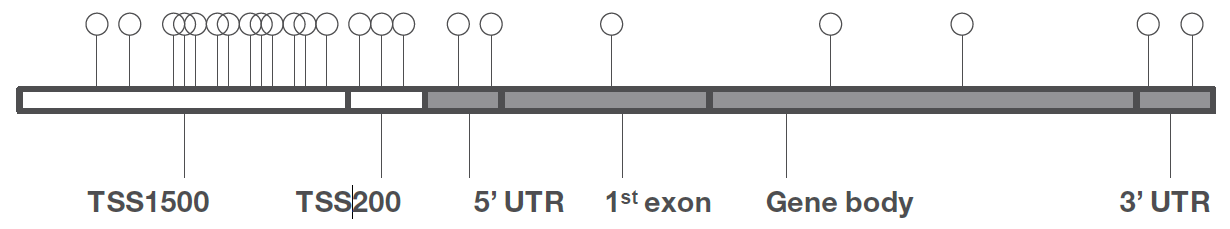
\includegraphics[width=7cm]{figures/Capture3.png}}
\end{center}
\begin{center}
    \fbox{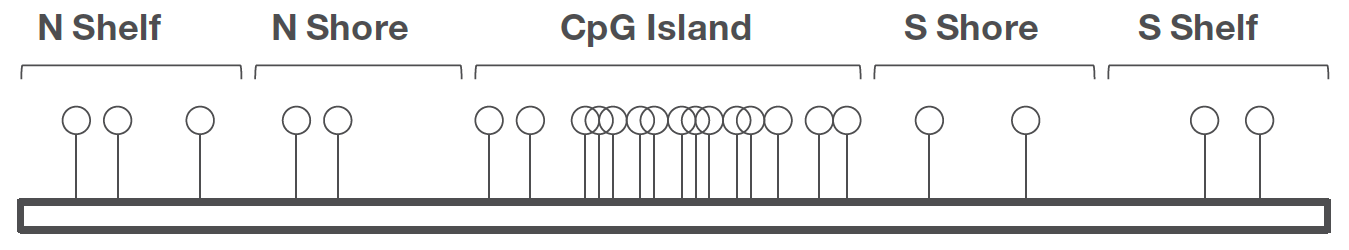
\includegraphics[width=7cm]{figures/Capture4.png}}
\end{center}
\end{frame}

\begin{frame}[allowframebreaks]{\blue{\lettrine{M}}éthodes \& Analyses}
\par{Au sein de la puce HumanMethylation450, deux technologies différentes sont utilisées pour mesurer le niveau de méthylation d'un site.}
\begin{minipage}[t]{0.475\columnwidth}
    \vspace{0.2cm}
    \begin{center}
        \fbox{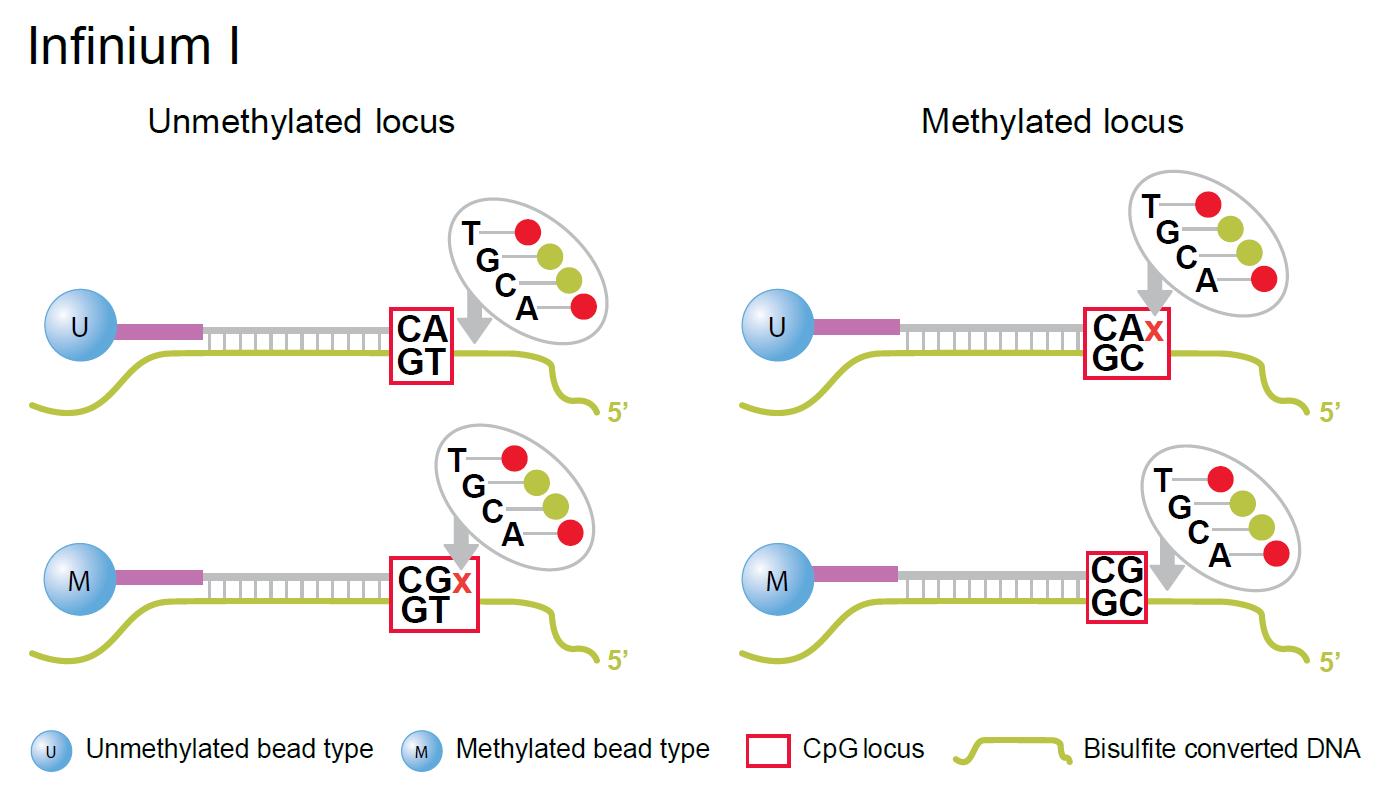
\includegraphics[width=5.5cm]{figures/Capture5.png}}
    \end{center}
\end{minipage}%
\hfill
\begin{minipage}[t]{0.475\columnwidth}
    \vspace{0.5cm}
    \begin{center}
        \fbox{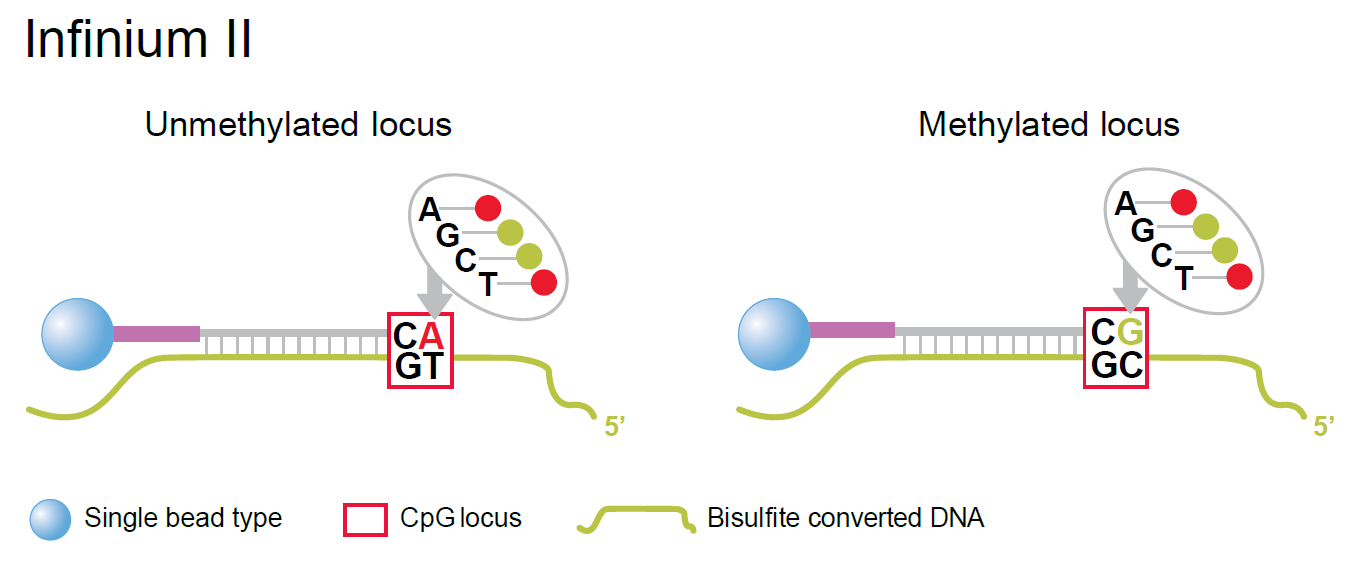
\includegraphics[width=5.5cm]{figures/Capture6.png}}
    \end{center}
\end{minipage}%
\framebreak
\par{Deux technologies? Deux mesures différentes...}
\par{Une étape de normalisation est donc nécessaire pour prendre en compte ce paramètre.}
\begin{center}
    \fbox{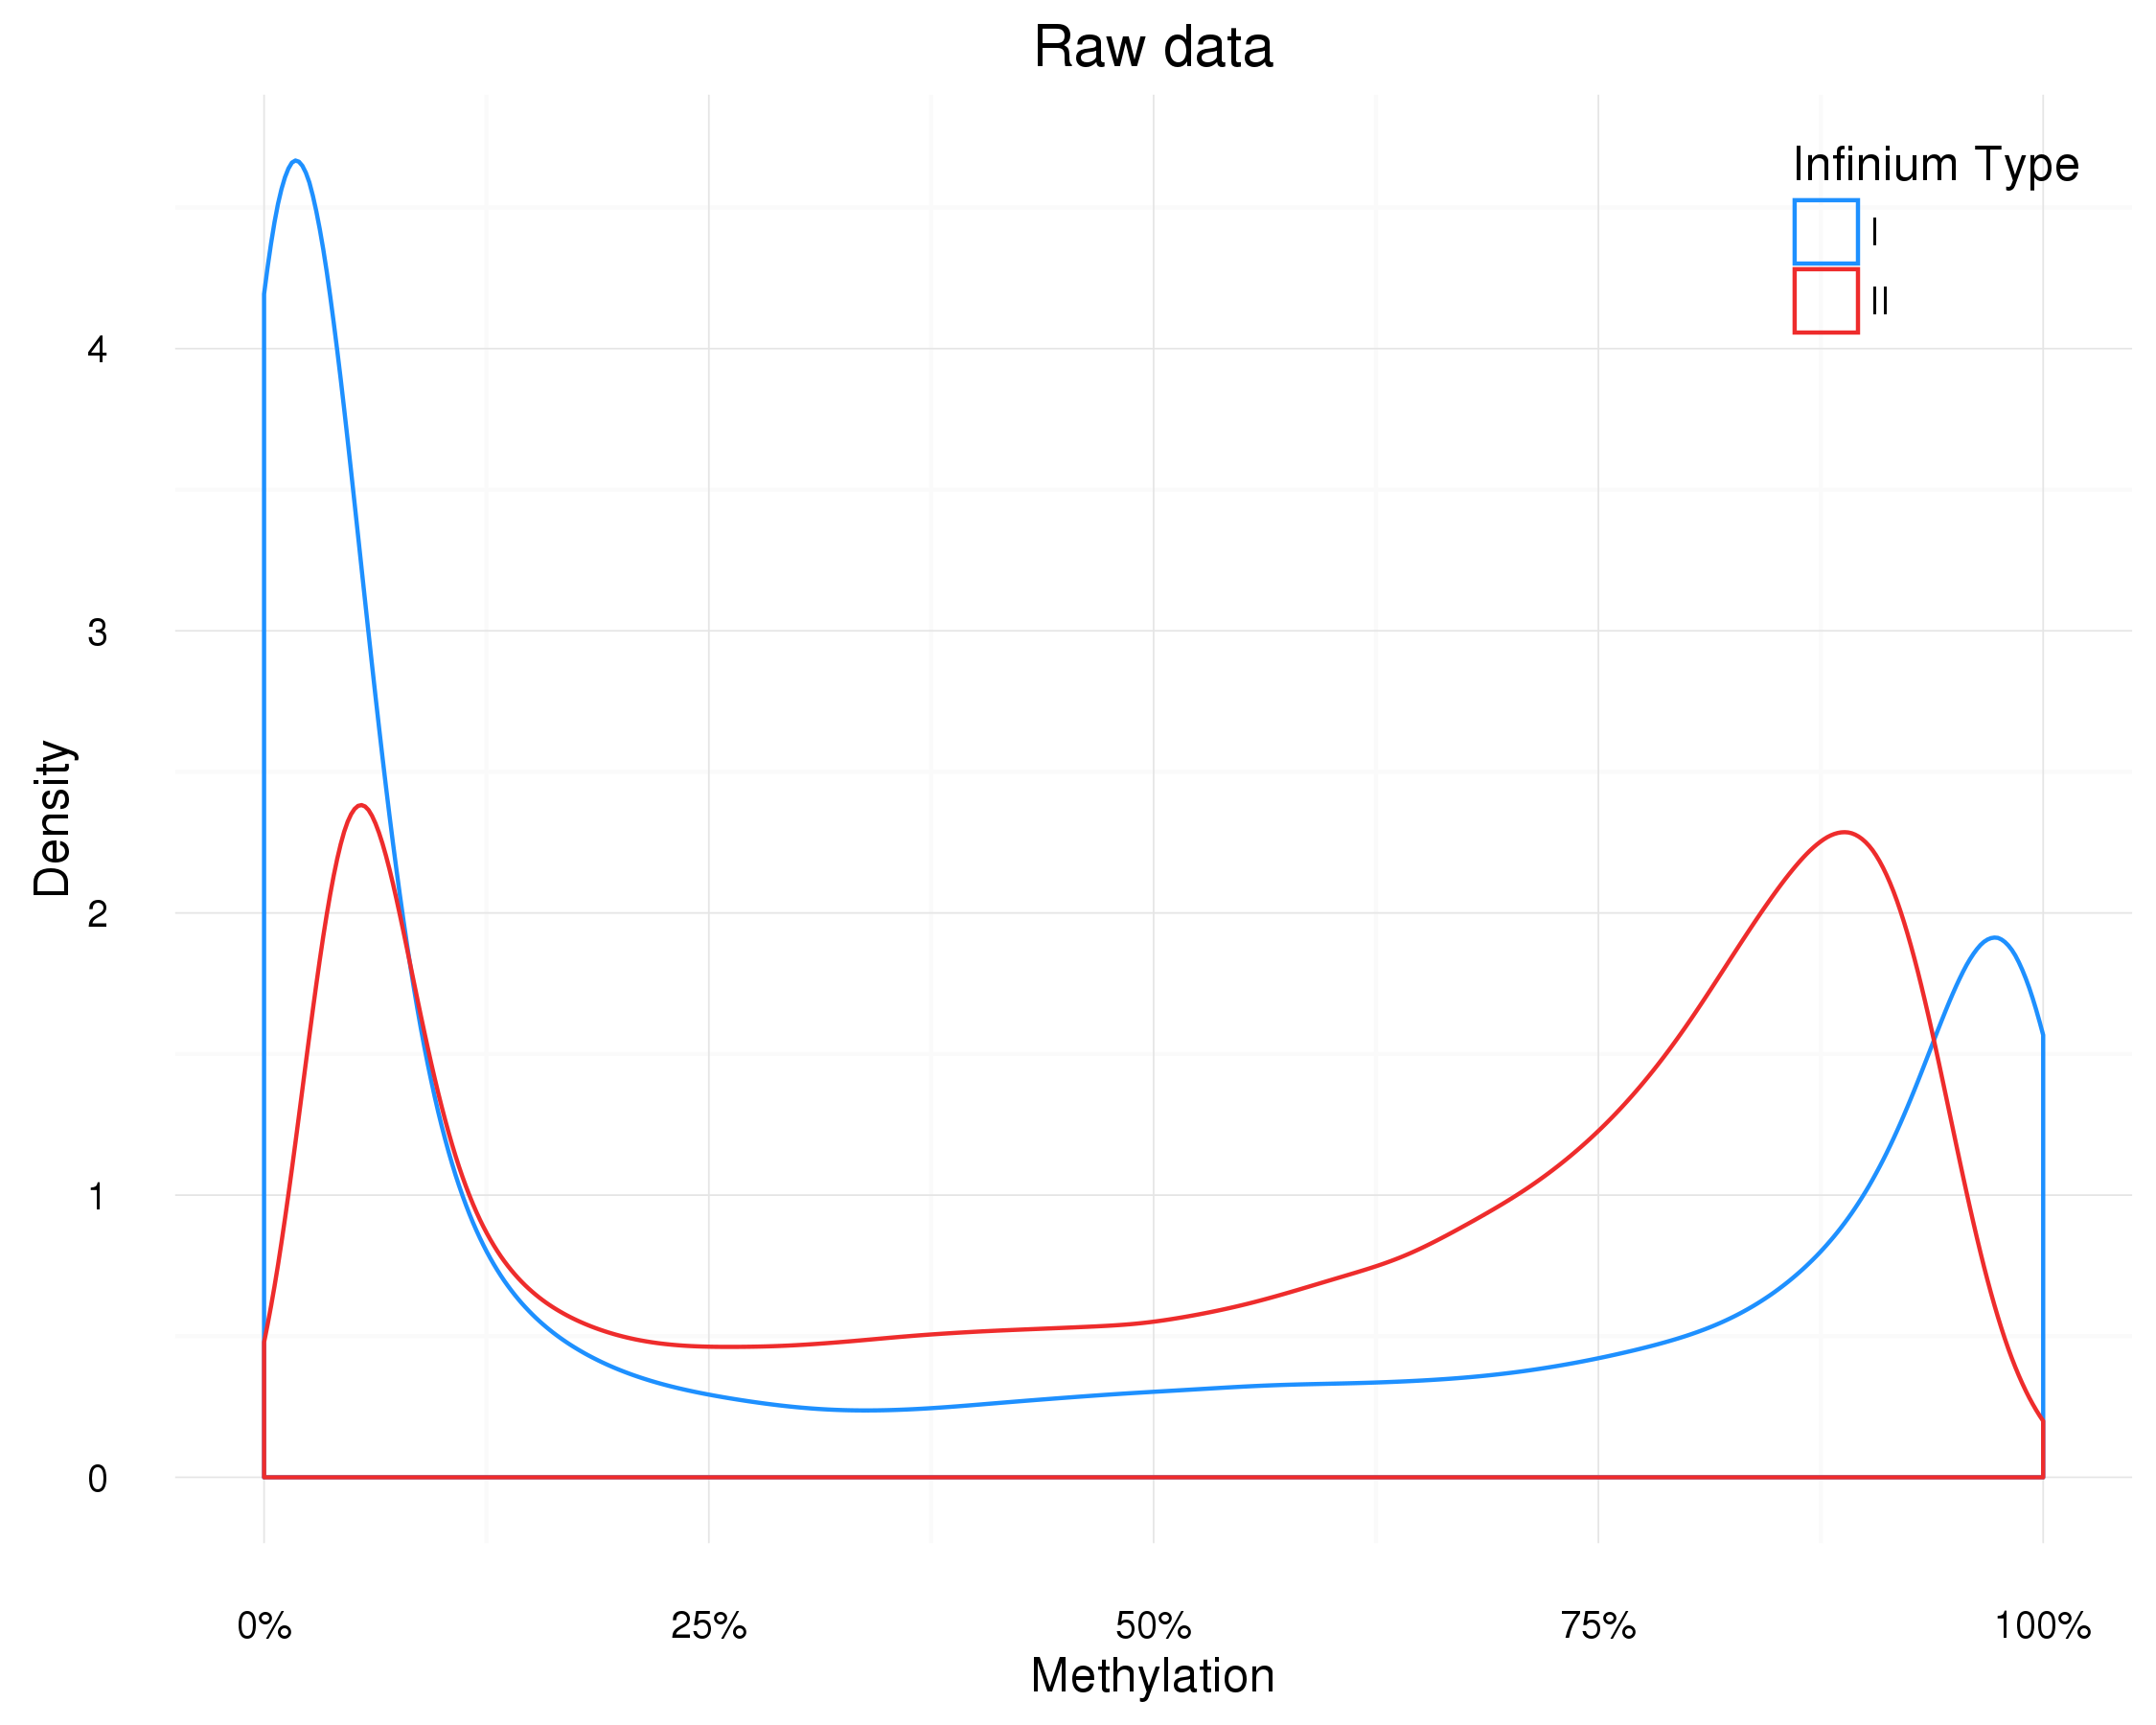
\includegraphics[width=5.5cm]{figures/InfiniumType_RawData.png}}
    \fbox{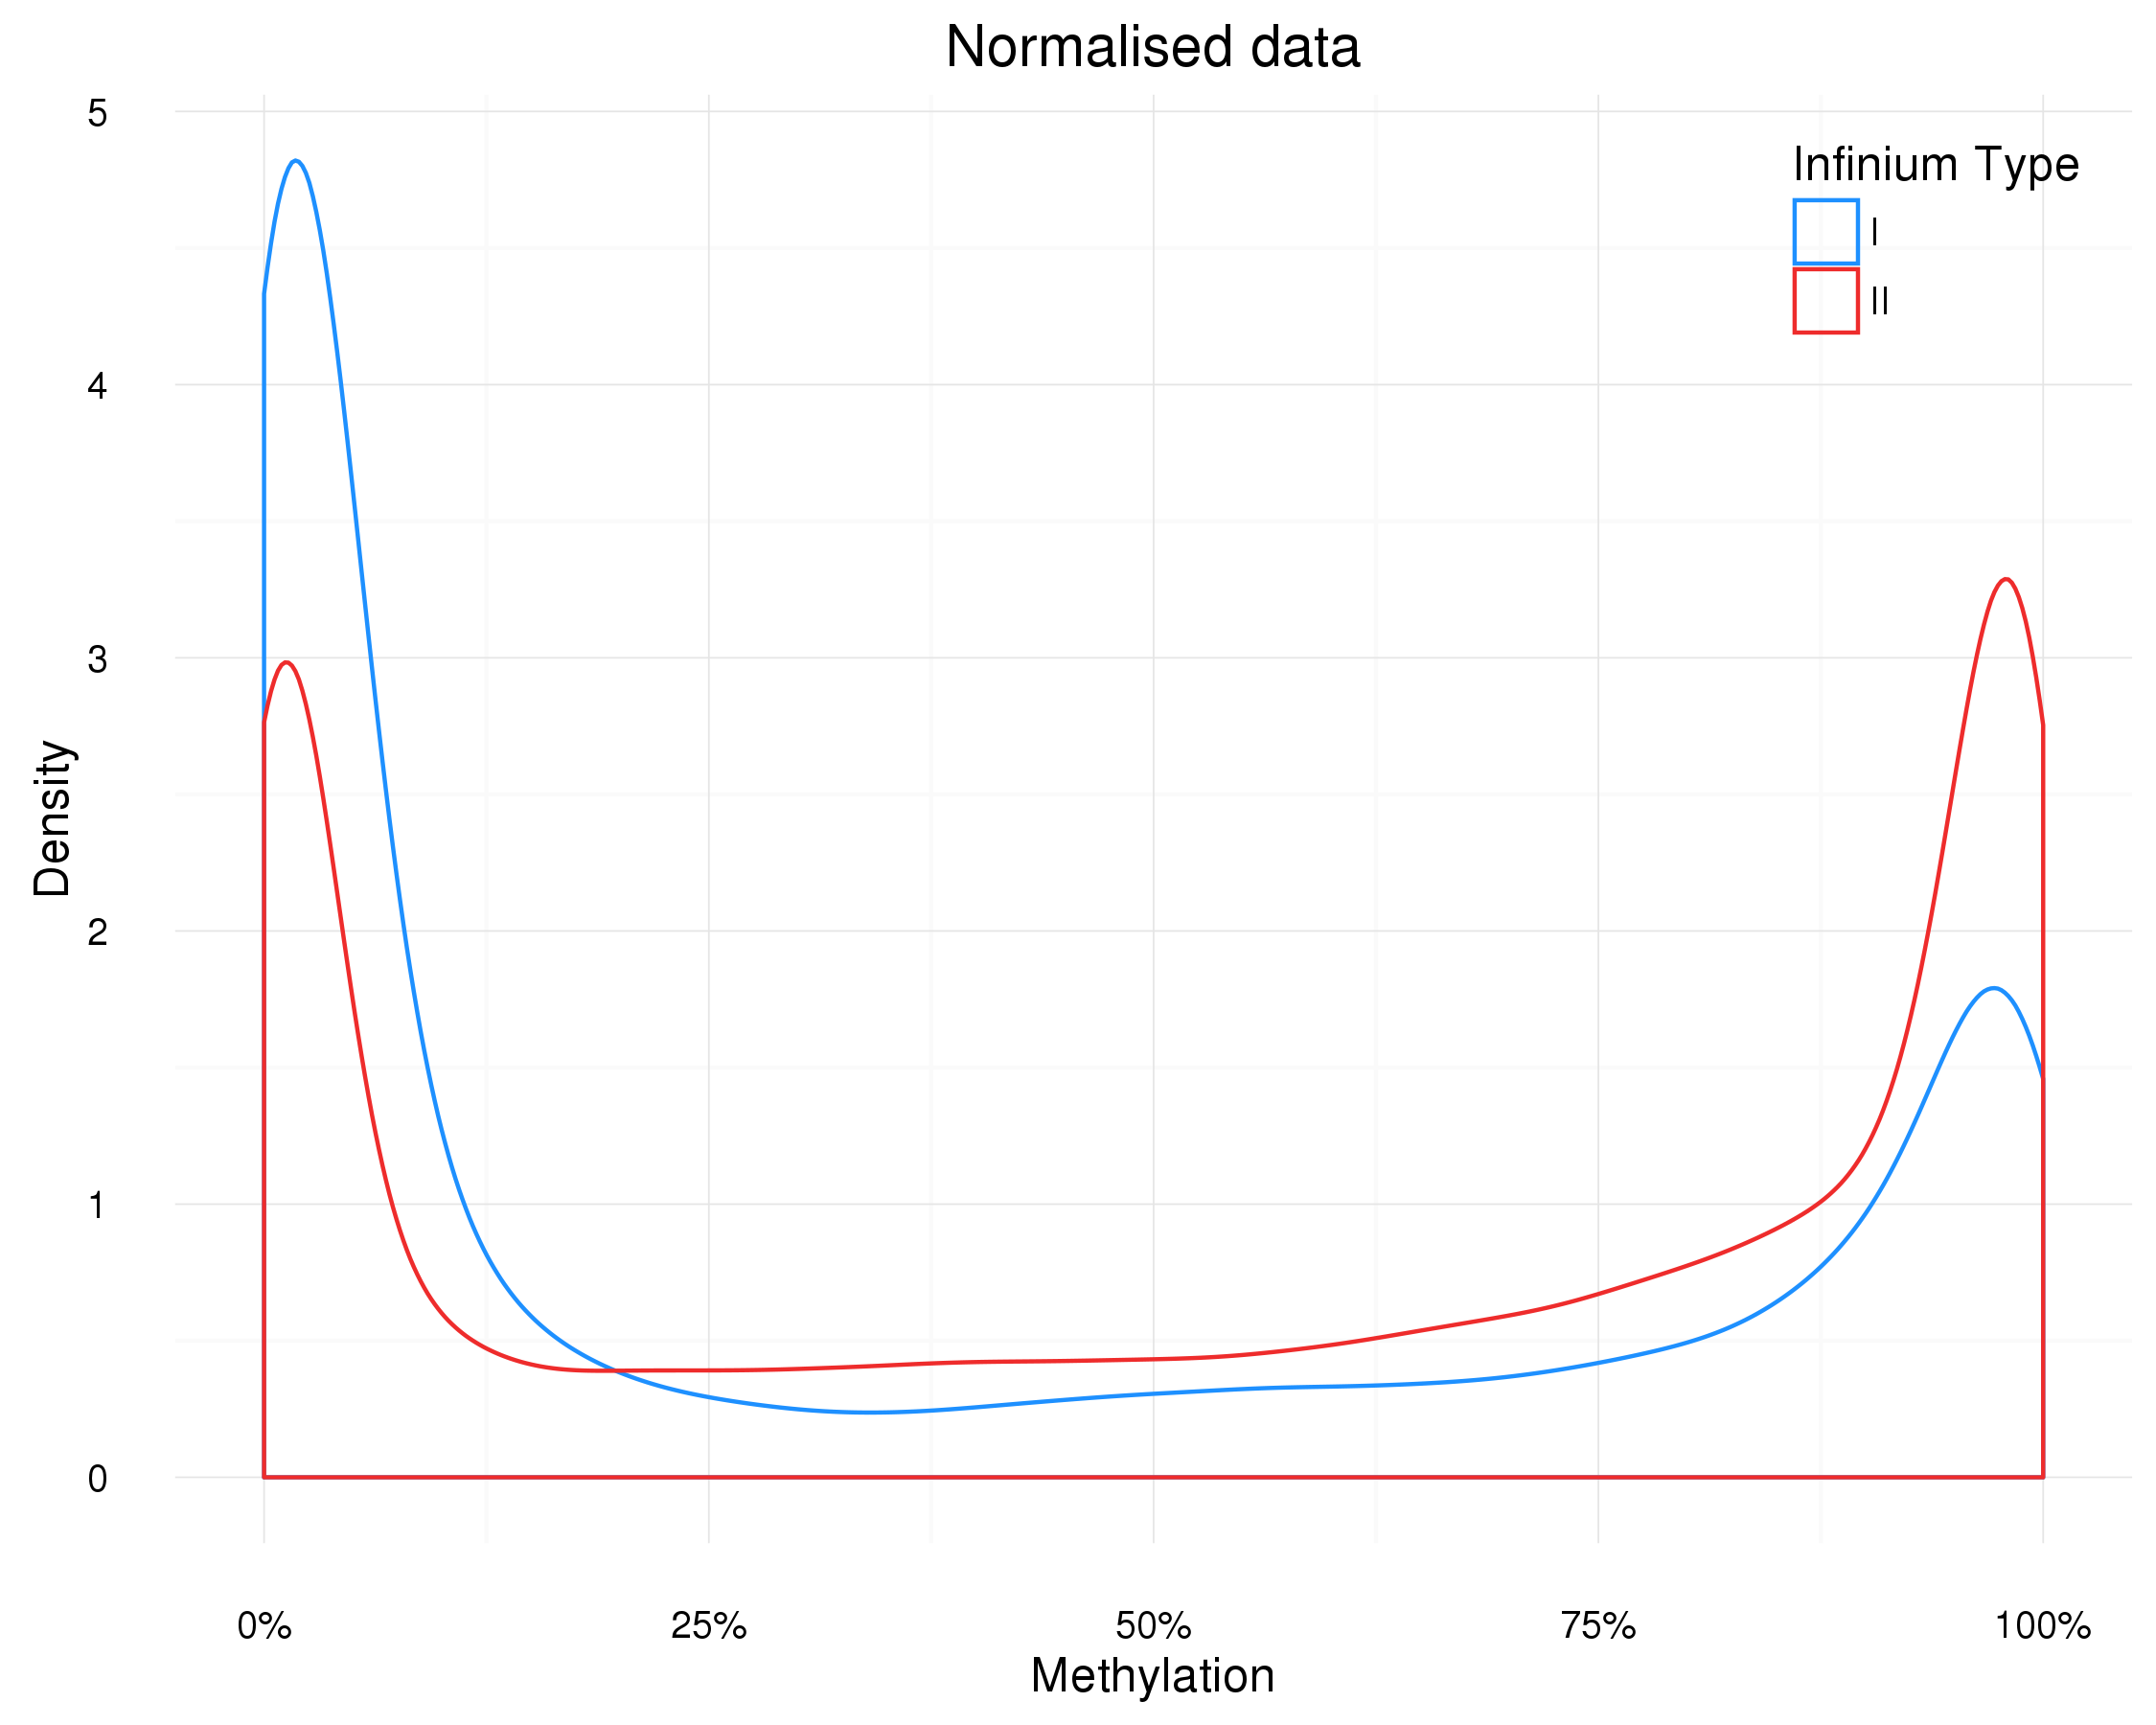
\includegraphics[width=5.5cm]{figures/InfiniumType_NormData.png}}
\end{center}
\framebreak
\par{Un autre paramètre technique pouvant induire un biais est:\newline l'effet plaque, le fameux "Batch Effect".}
\begin{center}
    \fbox{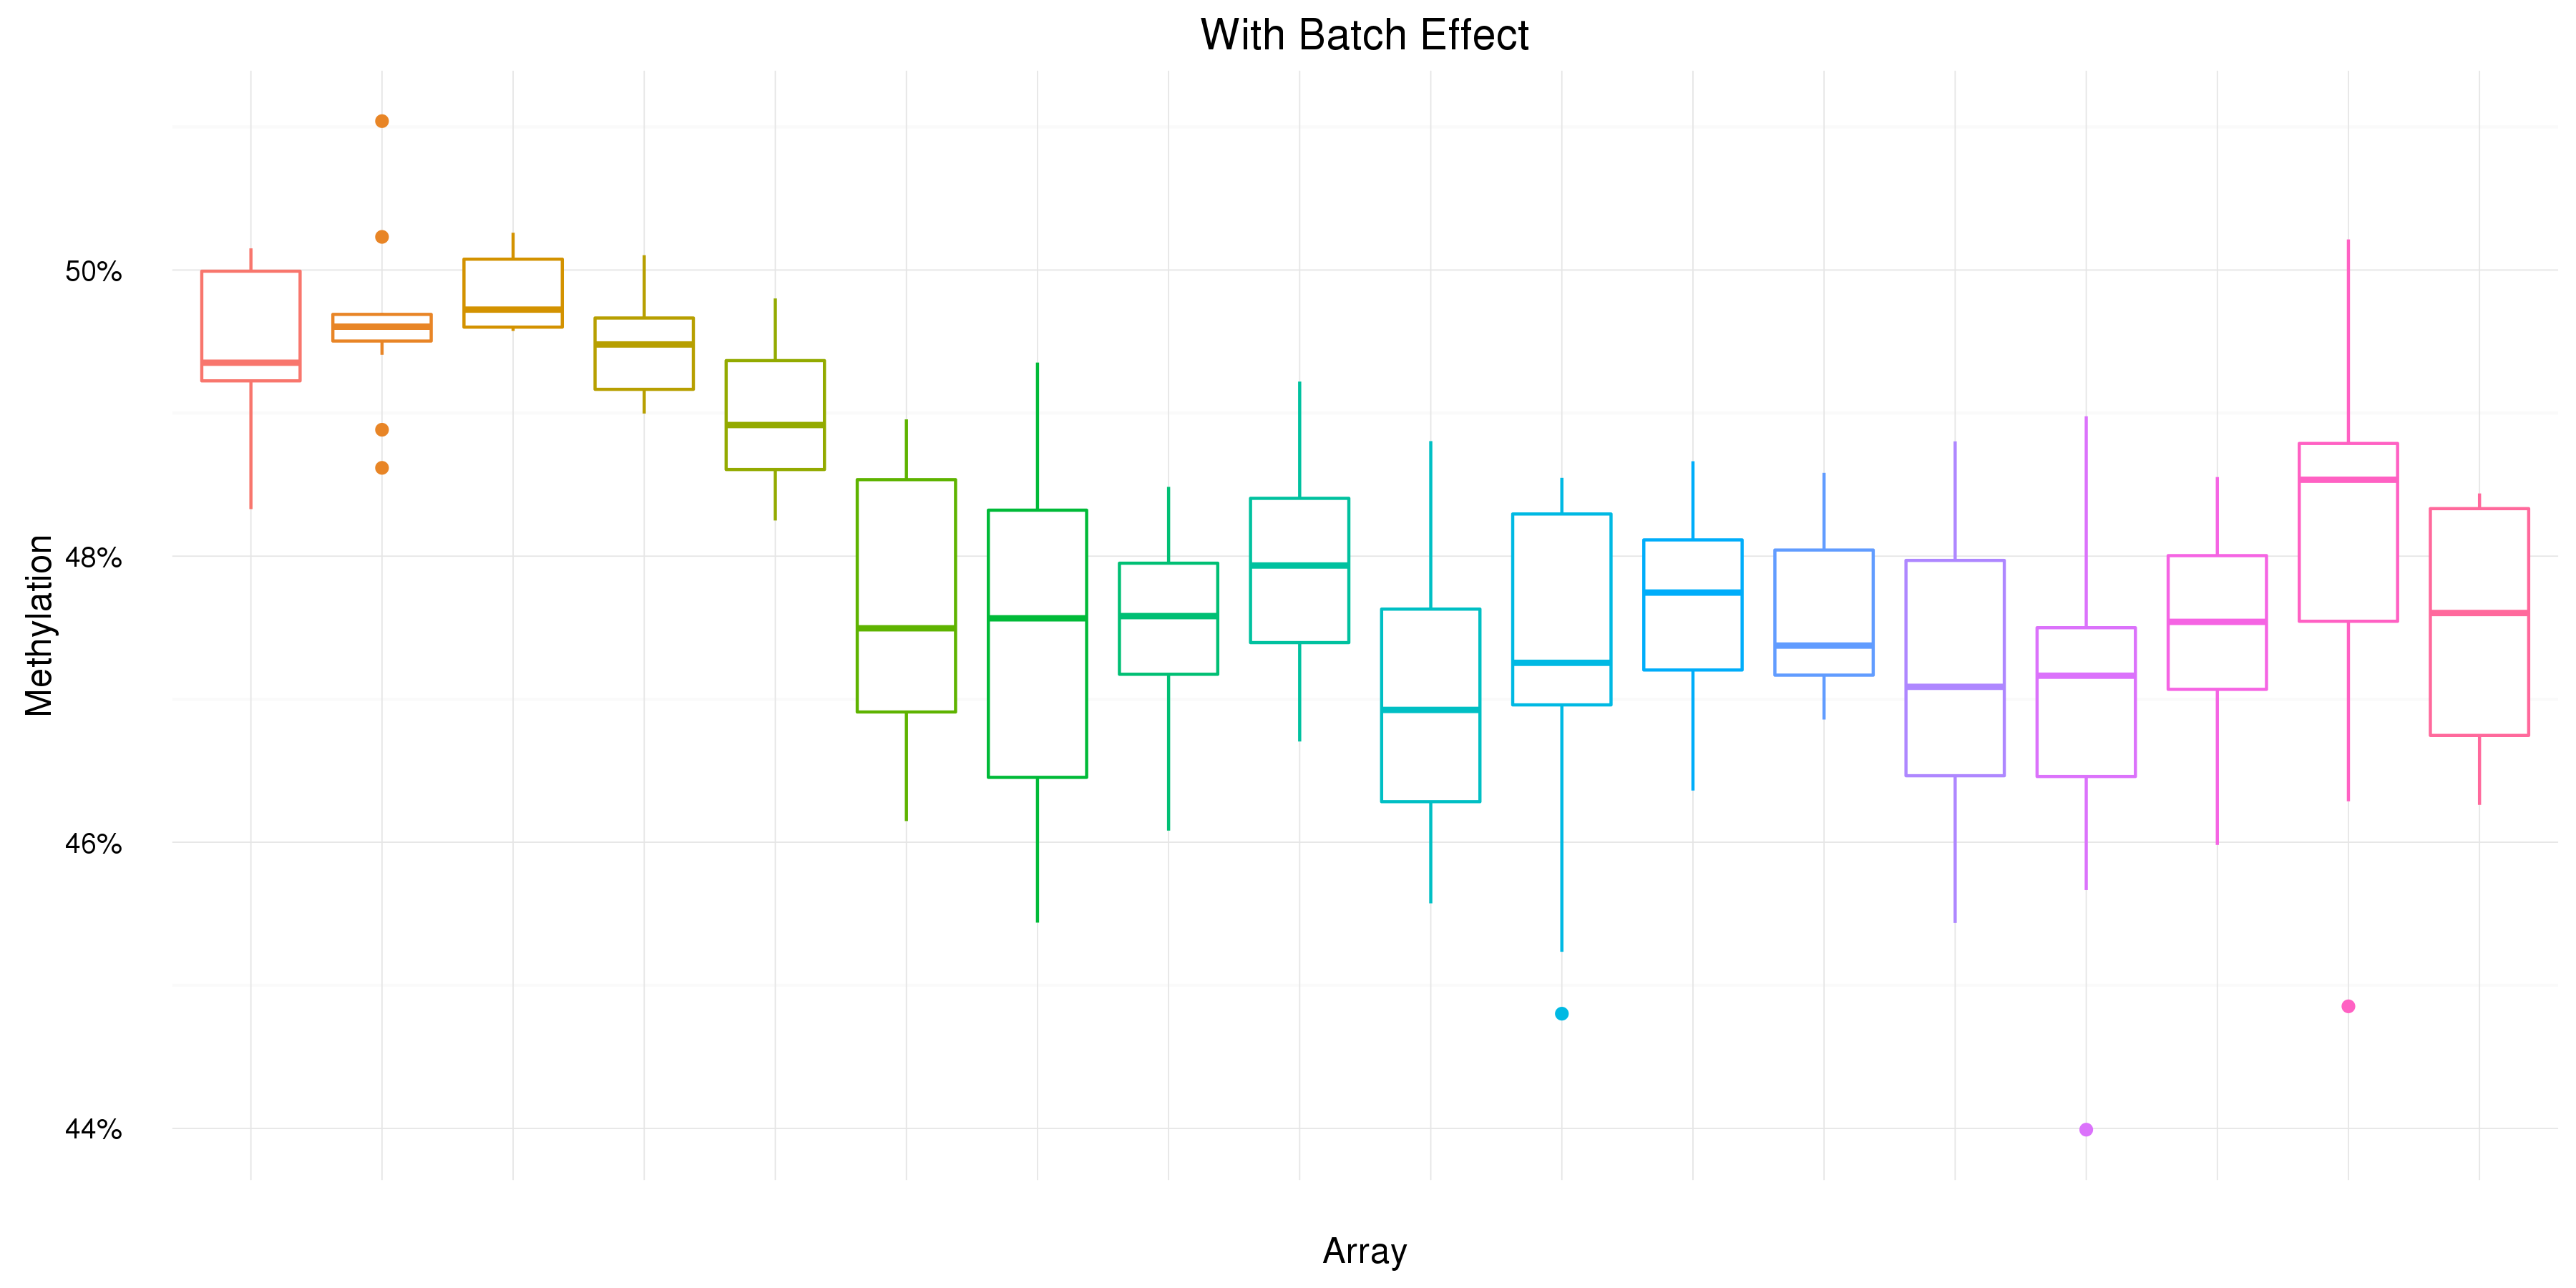
\includegraphics[width=5.5cm]{figures/BatchEffect_BatchData.png}}
    \fbox{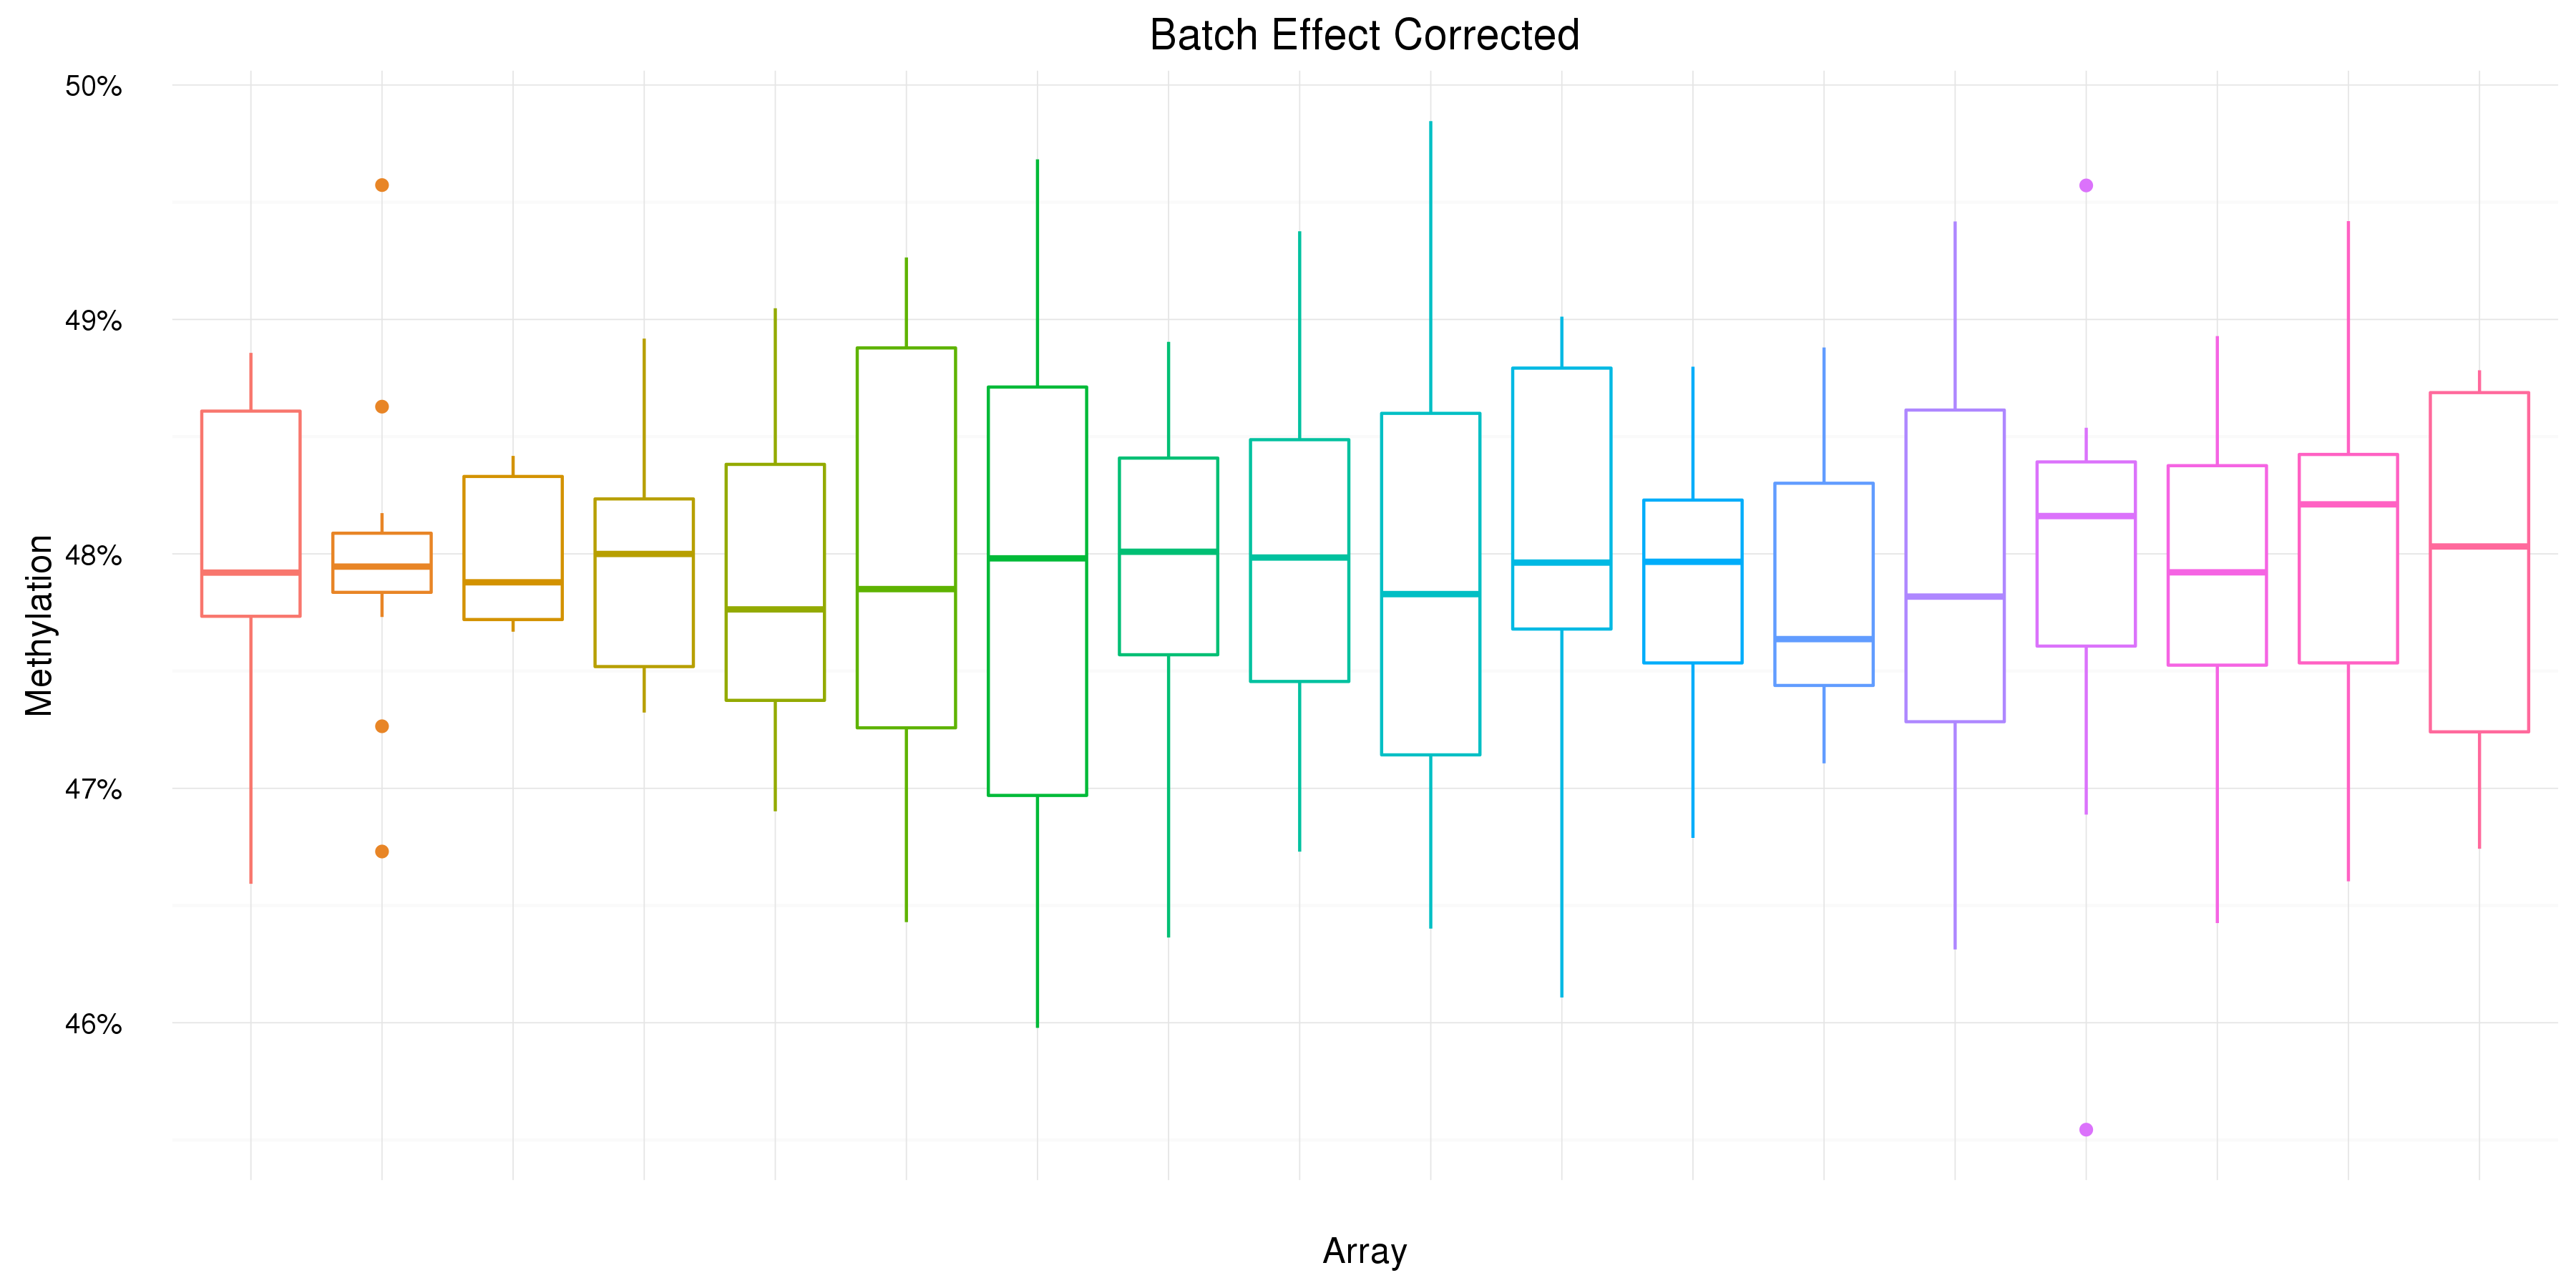
\includegraphics[width=5.5cm]{figures/BatchEffect_NoBatchData.png}}
\end{center}
\par{Une fois les données "propres", nous pouvons répondre à la problématique: ici un cas/contrôle.}
\par{Faisons simple, utilisons une régression linéaire de la forme:
\begin{eqnarray}Y = \theta_{0}+\theta_{1}\times X + \gamma \times Z\nonumber\end{eqnarray}
Avec:
\begin{description}
\item[Y] le niveau de notre site de méthylation compris entre 0 et 1,
\item[X] le statut de nos individus (0: contrôle; 1: cas),
\item[Z] des covariables comme l'âge, le sexe ou l'IMC,
\item[$\theta_0$, $\theta_1$, $\gamma$] les effets estimés.
\end{description}
}
\framebreak
\par{Après avoir effectué pas moins de 500 000 régressions linéaires, nous obtenons un tableau du même nombre de lignes...}
\vspace{1cm}
\par{Quelques mesures de précautions sont alors de rigueurs:}
\begin{itemize}
    \item Regarder le QQplot (quantile-quantile) => Avons-nous quelque-chose de systématique dans les résultats?
    \item Corriger les valeurs p ("p-value") pour les tests multiples => Le hasard n'est-il pas le seul responsable?
\end{itemize}
\framebreak
\par{Le QQ-plot, ça ressemble à quoi? Que nous dit ce graphique?}
\begin{center}
    \fbox{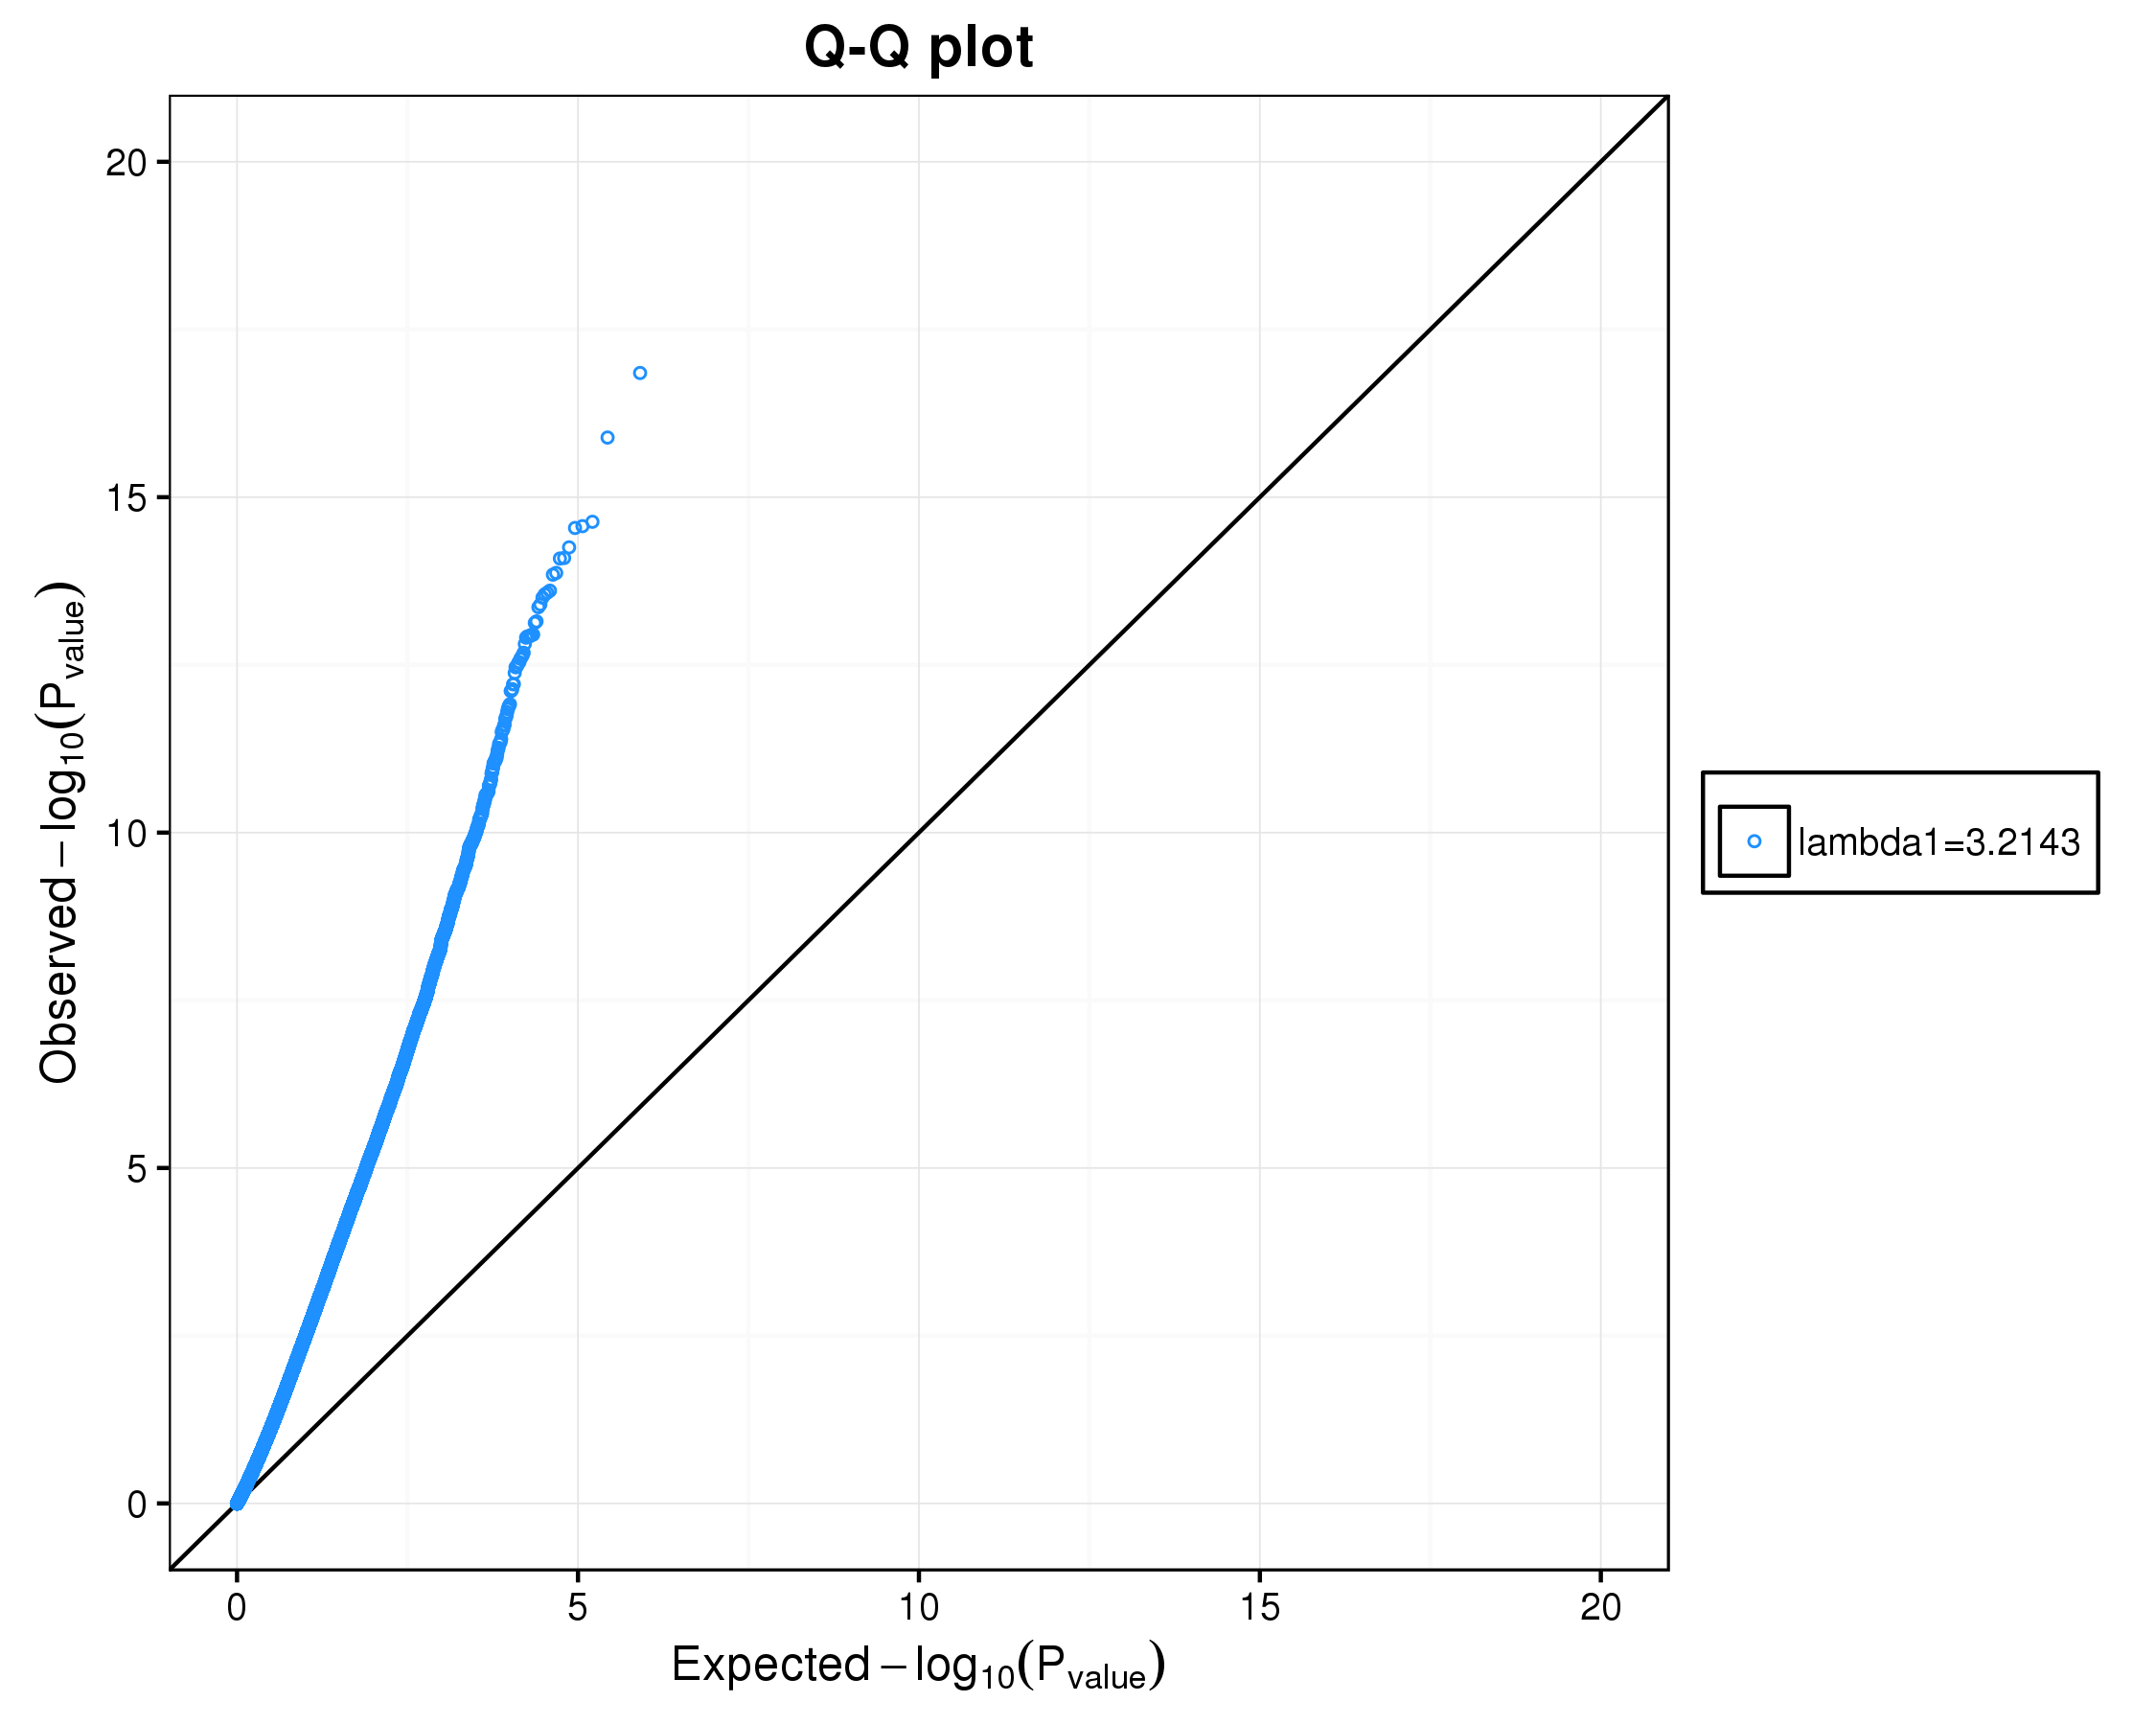
\includegraphics[width=7cm]{figures/QQplot.png}}
\end{center}
\framebreak
\par{Comment pouvons-nous corriger et savoir si le hasard est la cause de tous les maux?}
\vspace{1cm}
\par{La méthode la plus répandue et aussi la plus simple à mettre en oeuvre est la correction dite de Bonferroni.}
\framebreak
\par{Prenons un exemple, avec un seuil de significativité $\alpha=0.05$:}
\begin{center}
    \begin{tabular}{cccc}
        \hline
        CpG & Estimée & Valeur p & Significatif\\
        \hline
        CpG1 & 0.002315 & 0.1619 & Non\\
        CpG2 & 0.006276 & 0.00363 & Oui\\
        CpG3 & 0.004945 & 0.09727 & Non\\
        CpG4 & -0.04647 & 6.212e-06 & Oui\\
        CpG5 & 0.01847 & 0.04925 & Oui\\
        \hline
    \end{tabular}
\end{center}
\framebreak
\par{La correction de Bonferroni consiste à diviser notre seuil $\alpha=0.05$, par le nombre de tests effectuer (n=5), le nouveau seuil est donc $\alpha=0.05/5=0.01$:}
\begin{center}
    \begin{tabular}{cccc}
        \hline
        CpG & Estimée & Valeur p & Significatif\\
        \hline
        CpG1 & 0.002315 & 0.1619 & Non\\
        CpG2 & 0.006276 & 0.00363 & Oui\\
        CpG3 & 0.004945 & 0.09727 & Non\\
        CpG4 & -0.04647 & 6.212e-06 & Oui\\
        CpG5 & 0.01847 & 0.04925 & Non\\
        \hline
    \end{tabular}
\end{center}
% \par{Ainsi, pour réduire le risque de faux-positif (lié au hasard) dans les résultats, le seuol de significative ($\alpha$) est abaissé, ce qui a pour conséquence de faire disparaître "CpG5" dans l'exemple.}
\framebreak
\par{Une représentation de ces résultats serait le "Manhattan plot".}
\begin{center}
    \fbox{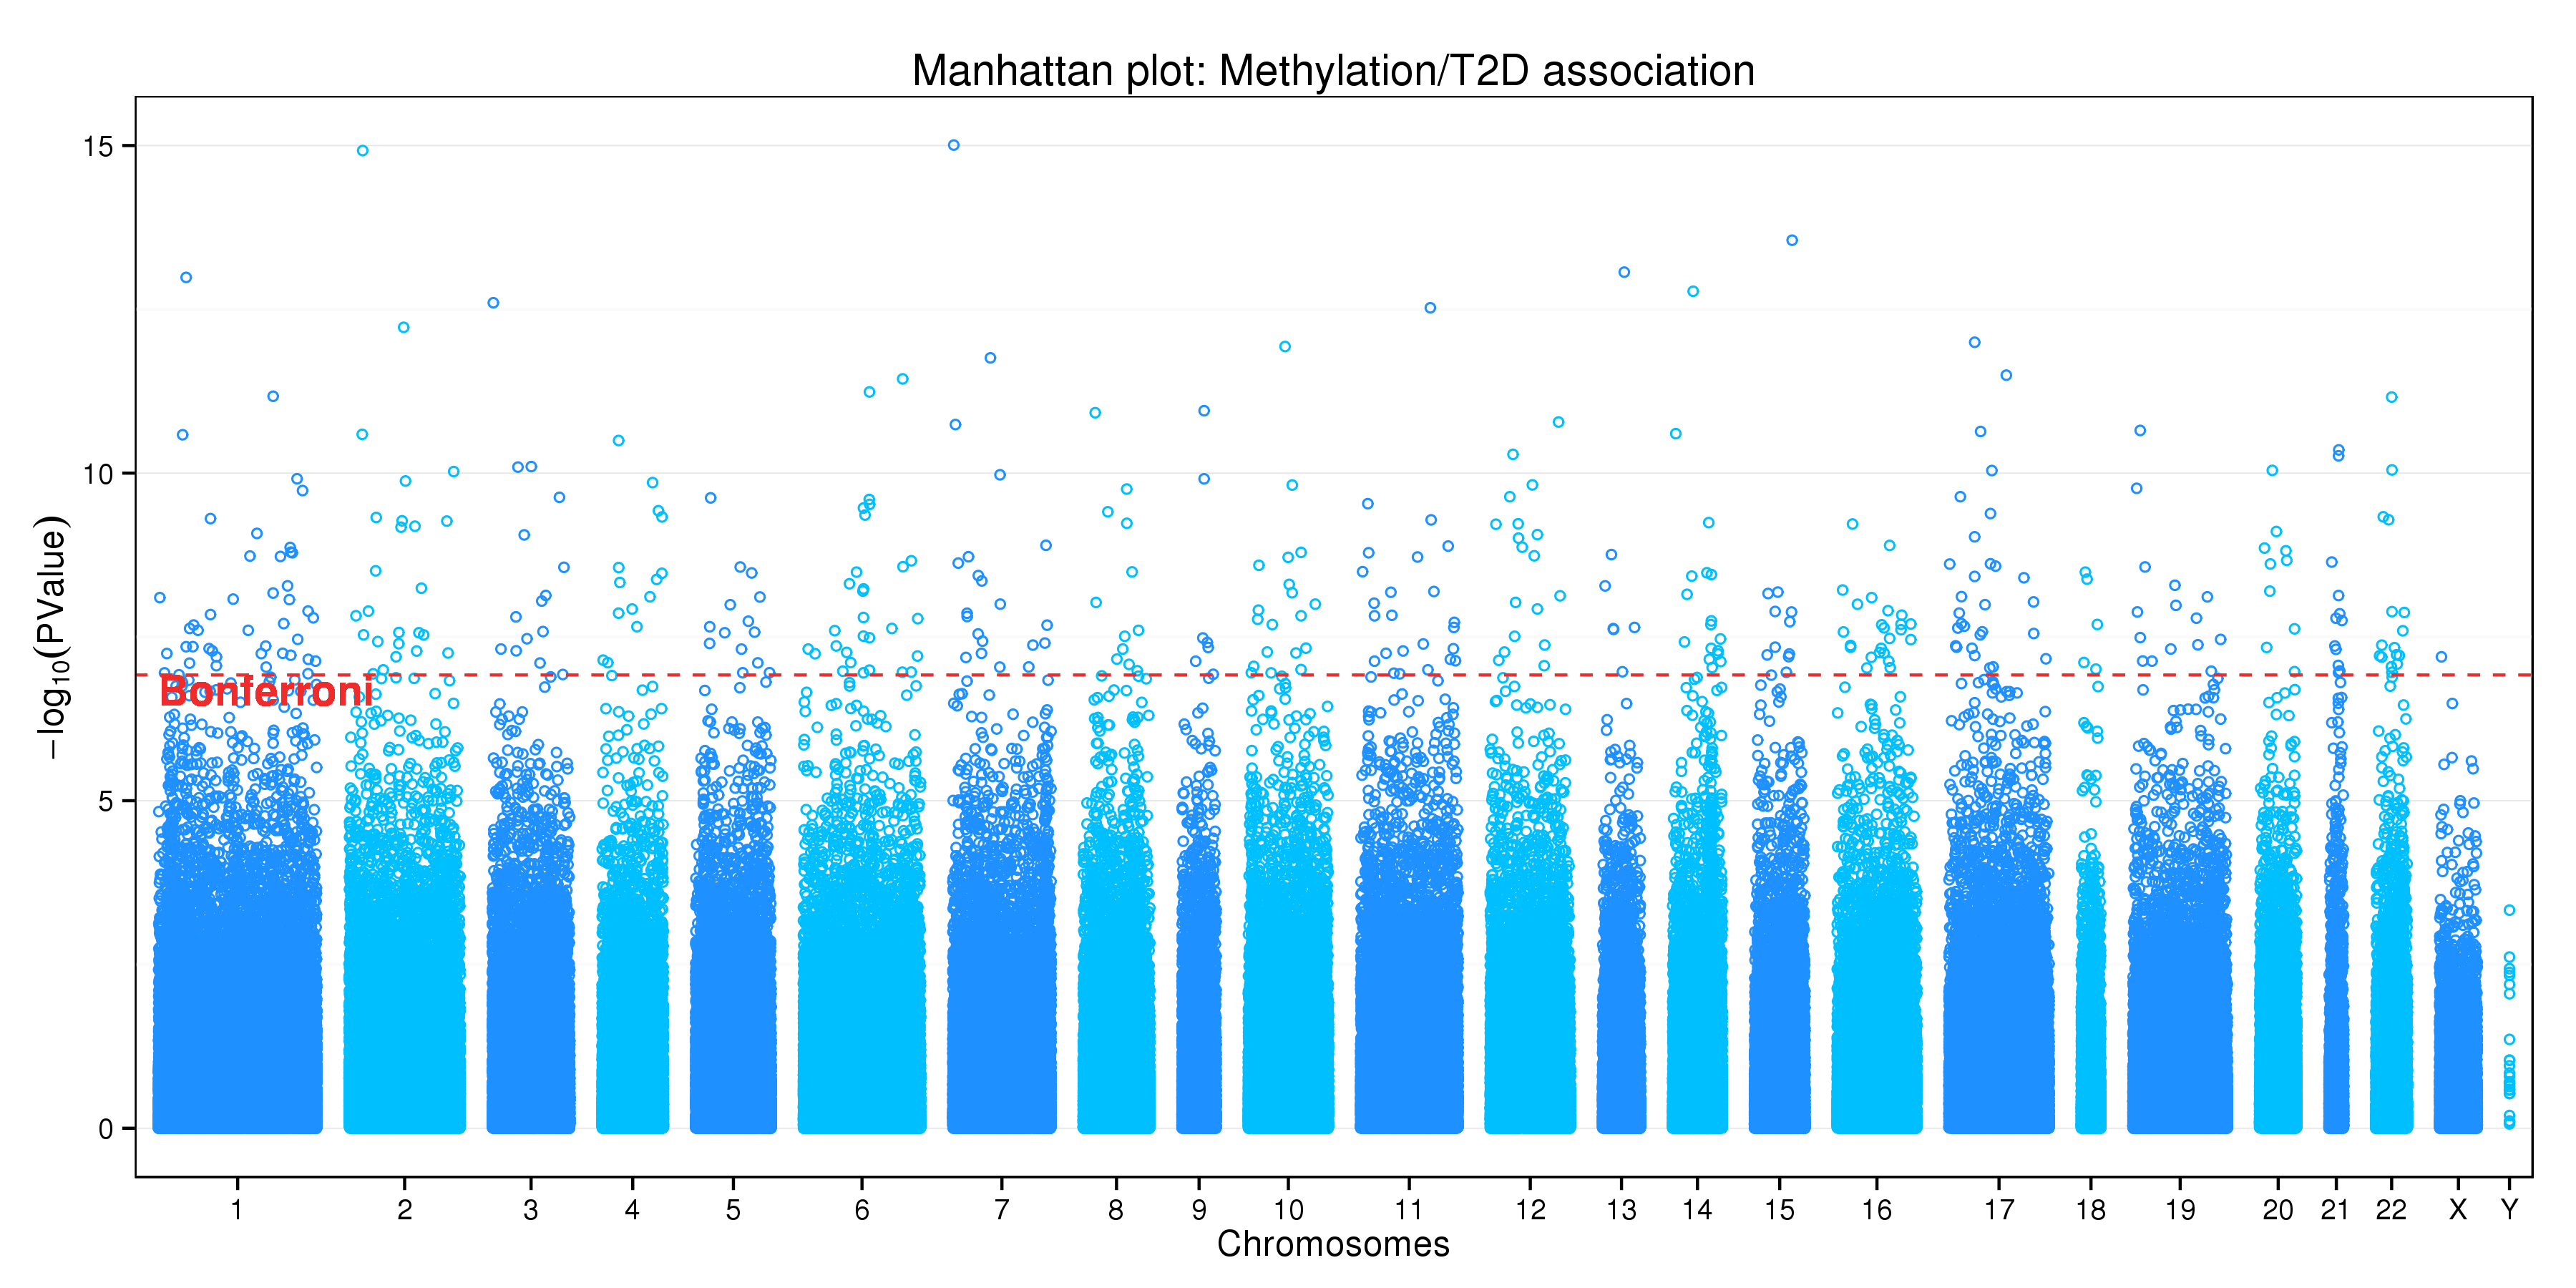
\includegraphics[width=9cm]{figures/Methylation_ManhattanPlot_Association_T2D.png}}
\end{center}
\framebreak
\par{La puissance statistique (ou du statisticien)!}
\begin{center}
    \fbox{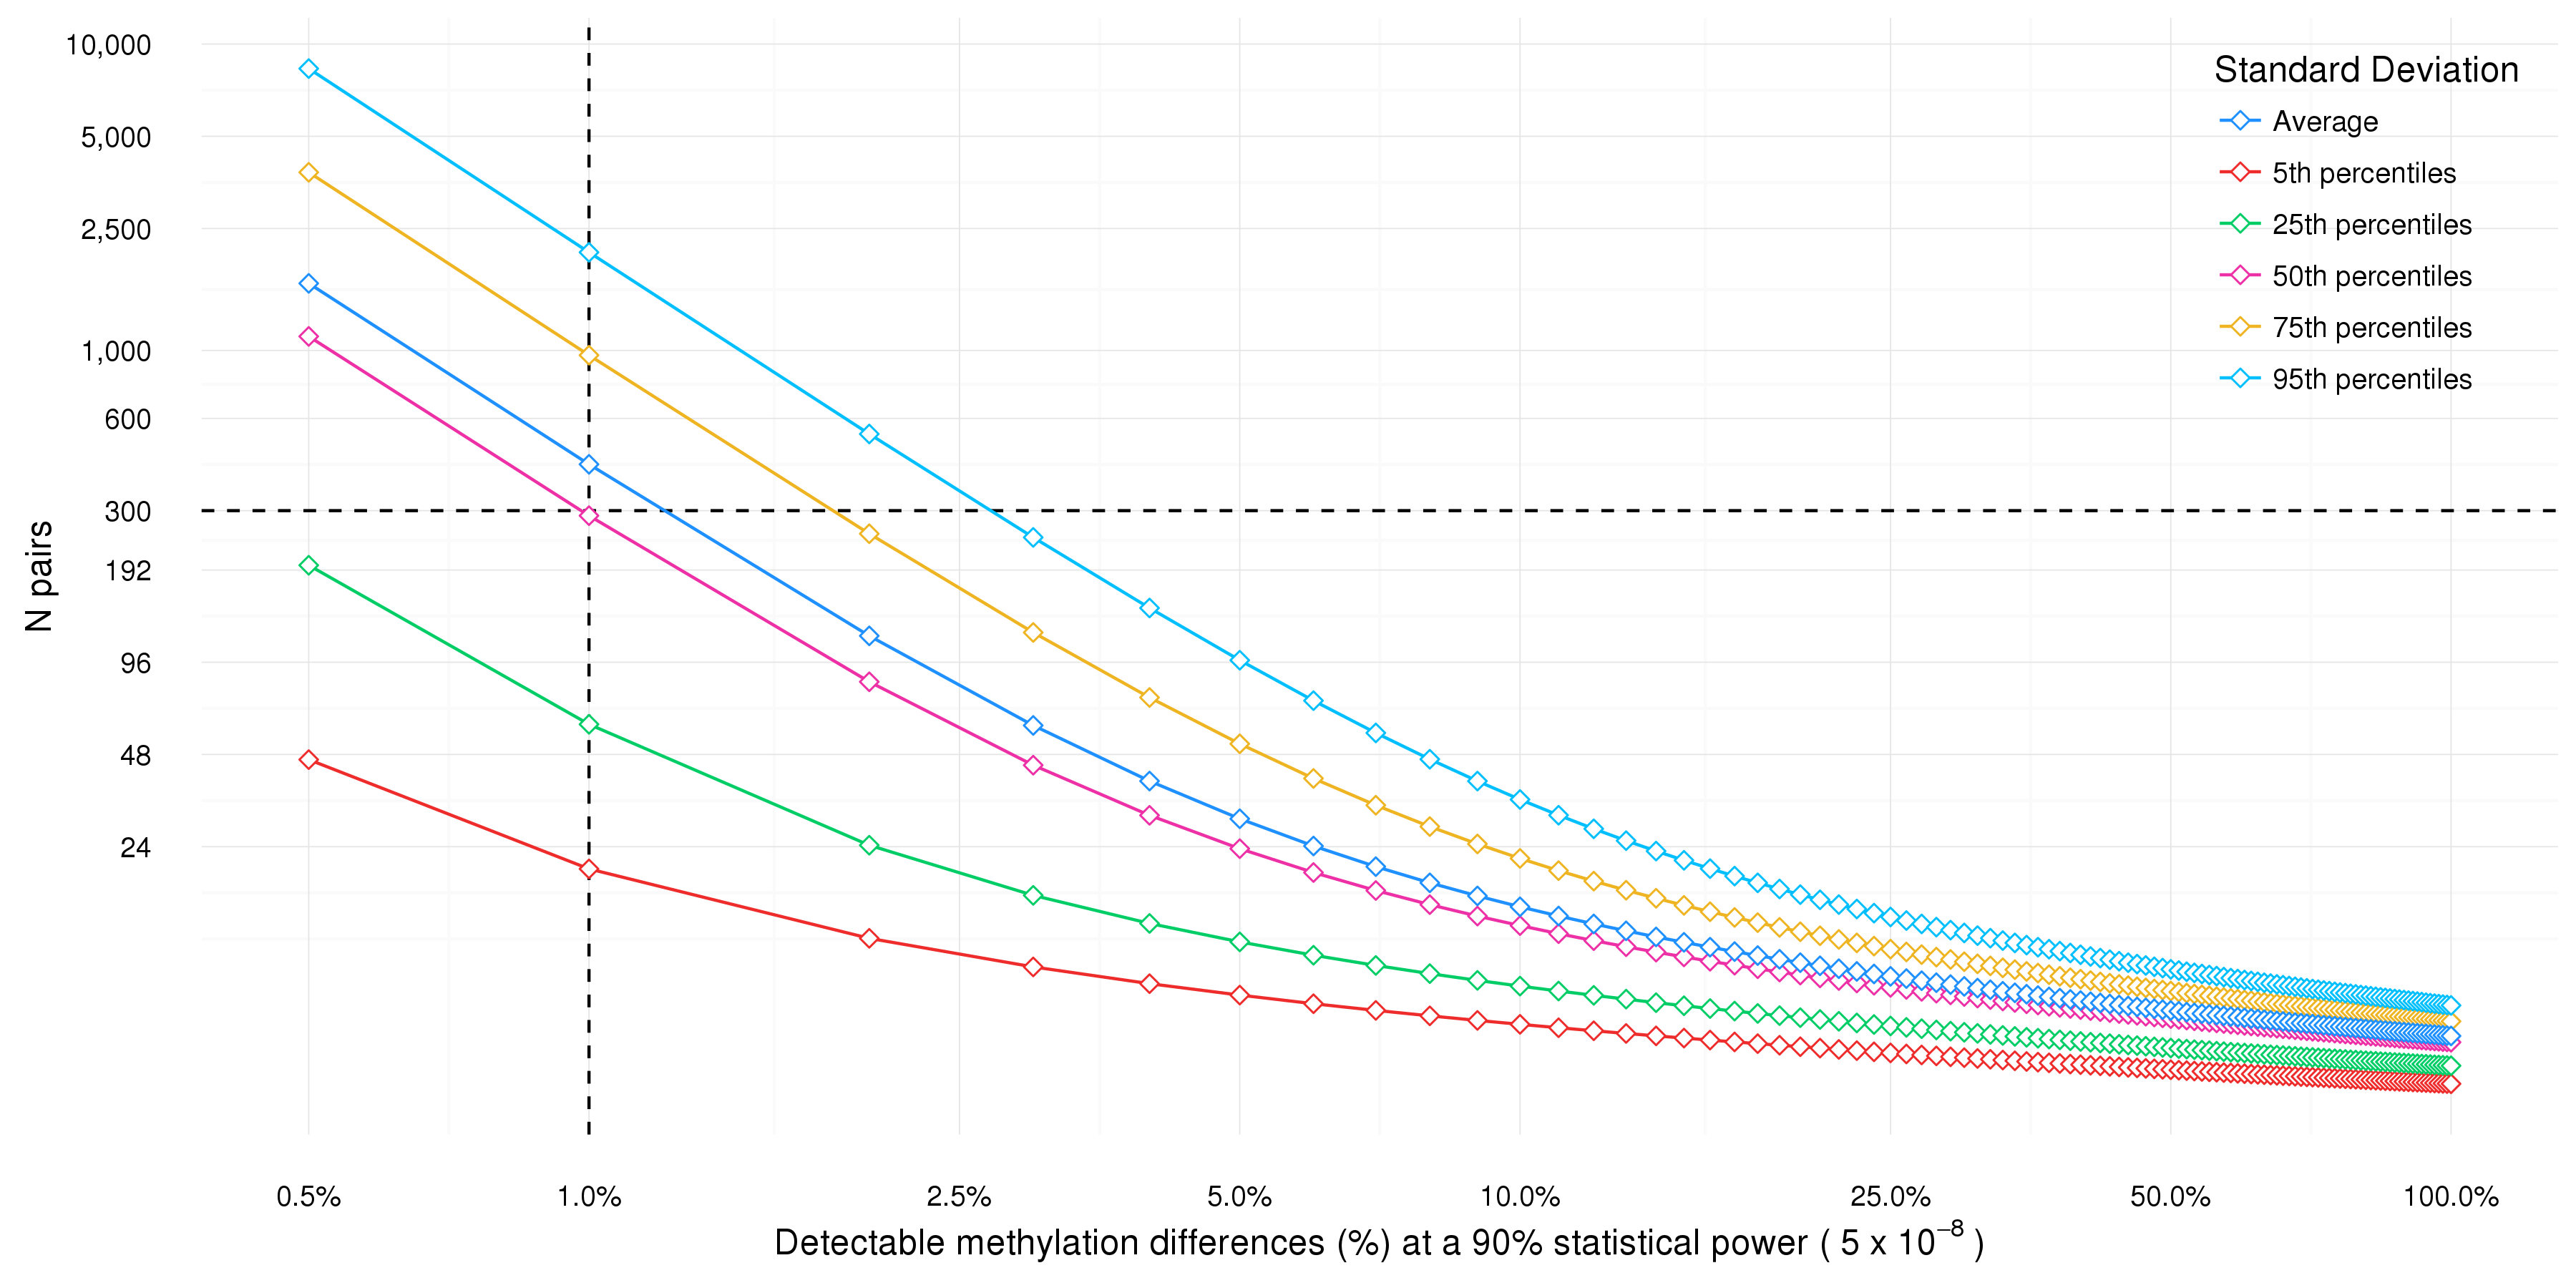
\includegraphics[width=9cm]{figures/MethylPowerStudy.png}}
\end{center}
\end{frame}

\begin{frame}[allowframebreaks]{}
    \begin{center}
        \huge {\rmfamily \textbf{``}}\textcolor{dodgerblue}{The best thing about being a statistician is that you get to play in everyone's backyard}{\rmfamily \textbf{''}}\vspace{-1em}\begin{flushright}--- John Tukey\end{flushright}
    \end{center}
\end{frame}

% \section{Références}
% \begin{frame}<beamer:0>{\blue{\lettrine{R}}éférences}
    % \bibliographystyle{apalike}
    % \bibliography{JTLille2.bib}
% \end{frame}


\end{document}